%***********************************************************
% zewwww Paper Template
% Simon Reif & Benedikt Stelter, 19 September 2024
%
% Preamble
% This tex code is use to be run together with the
% corresponding Quarto file.
%***********************************************************

% Packages
\documentclass[12pt,a4paper,oneside]{article} % Layout
\usepackage[utf8]{inputenc}
\usepackage[british]{babel}
\usepackage{graphicx,txfonts} % Even more symbols
\usepackage[T1]{fontenc}
\usepackage[onehalfspacing]{setspace}
\usepackage[strict=true, style=american]{csquotes}
\usepackage[lmargin=1.2in,rmargin=1.2in,tmargin=1.2in,bmargin=1.2in]{geometry}
\usepackage{float}
\usepackage{multirow}
\usepackage{longtable}
\usepackage{colortbl}
\usepackage{booktabs}
\usepackage{threeparttable}
\usepackage{subcaption}
\usepackage[dvipsnames]{xcolor}
\usepackage{fontspec}
\usepackage{amssymb} % Extra symbols
\usepackage{titling}
\usepackage[style=apa]{biblatex}
\usepackage[linktoc=all, colorlinks=true]{hyperref}
\usepackage{placeins}


% Use packages from YMAL header:
\usepackage{bm}
\usepackage{setspace}
\usepackage{lipsum}

% Set text format
\setmainfont[BoldFont=LinLibertine_RB.ttf,
ItalicFont=LinLibertine_RI.ttf]{LinLibertine_R.ttf}
\definecolor{footnotecolor}{RGB}{82,125,164}

% Add new pandocbounced command to comply with pandoc update 3.5
\makeatletter
\newsavebox\pandoc@box
\newcommand*\pandocbounded[1]{% scales image to fit in text height/width
  \sbox\pandoc@box{#1}%
  \Gscale@div\@tempa{\textheight}{\dimexpr\ht\pandoc@box+\dp\pandoc@box\relax}%
  \Gscale@div\@tempb{\linewidth}{\wd\pandoc@box}%
  \ifdim\@tempb\p@<\@tempa\p@\let\@tempa\@tempb\fi% select the smaller of both
  \ifdim\@tempa\p@<\p@\scalebox{\@tempa}{\usebox\pandoc@box}%
  \else\usebox{\pandoc@box}%
  \fi%
}
\makeatother

% Unnecessary but nice: change symbols for title page notes
\makeatletter
\def\@fnsymbol#1{\ensuremath{\ifcase#1\or \varheartsuit \or \bigstar \or \dagger\or \ddagger\or
\mathsection\or \mathparagraph\or \|\or **\or \dagger\dagger
\or \ddagger\ddagger \else\@ctrerr\fi}}
\makeatother

\settowidth{\thanksmarkwidth}{*}
\setlength{\thanksmargin}{-\thanksmarkwidth}


% Add Bib file from YMAL Header
\addbibresource{../references.bib}

% Print references
 
\makeatletter
\@ifundefined{date}{}{\date{}}
\setcounter{page}{1}

\makeatletter
\renewcommand\@makefnmark{\hbox{\@textsuperscript{\normalfont\color{footnotecolor}\@thefnmark}}}
\renewcommand\@makefntext[1]{%
  \parindent 1em\noindent
            \hb@xt@1.8em{%
                \hss\@textsuperscript{\normalfont\@thefnmark}}#1}
\makeatother

% Make font size of minipage scriptsize by default s.t. table notes are small
\AtBeginEnvironment{minipage}{\scriptsize}

\hypersetup{
		pdftitle={zewwwwEcon: A Template for Econ Articles with Quarto},
			pdfauthor={First Author; Second Author; Third Author; Fourth Author},
					pdfkeywords={These are the keywords},
		colorlinks=true,
	linkcolor={[RGB]{82,125,164}},
	filecolor={[RGB]{82,125,164}},
	citecolor={[RGB]{82,125,164}},
	urlcolor={[RGB]{82,125,164}},
	pdfcreator={LaTeX via pandoc}}

\begin{document}

%***********************************************************
% Title page
%***********************************************************

\setlength{\droptitle}{-8em}  % Change whitespace above title
	\title{	\rule{\linewidth}{0.5mm} \textbf{
		{\LARGE zewwwwEcon: A Template for Econ Articles with
Quarto \vspace{-15pt} }}\thanks{\noindent { }We would like to thank
\ldots.}  \rule{\linewidth}{0.5mm}  }
\date{\hspace{87pt}\scriptsize{\textbf{Version
0.1 \#8098b377}} \vspace{-5pt} \newline  \normalsize 4 November 2024} 

\author{
		\textbf{First Author}\\
	\small{Affiliation A which is very long}\vspace{-1.5ex}\\
	\and	\textbf{Second Author}\thanks{ { }Corrseponding author: Adress,
Place.}\\
	\small{Affiliation B}\vspace{-1.5ex}\\
	\and	\textbf{Third Author}\\
	\small{Affiliation B}\vspace{-1.5ex}\\
	\small{Affiliation C}\vspace{-1.5ex}\\
	\and	\textbf{Fourth Author}\\
	\small{Affiliation B}\vspace{-1.5ex}\\
	\small{Affiliation C}\vspace{-1.5ex}\\
	\vspace{10pt}}

\maketitle
\thispagestyle{empty}

\begin{center}
\vspace{-25pt}	\noindent \textit{Preliminary draft - please do not
distribute}
\end{center}

\begin{abstract}
	\vspace{-15pt}	\singlespacing{
		\noindent O, never Shall sun that morrow see! Your face, my thane, is as
a book where men May read strange matters. To beguile the time, Look
like the time; bear welcome in your eye, Your hand, your tongue: look
like the innocent flower, But be the serpent under't. He that's coming
Must be provided for: and you shall put This night's great business into
my dispatch; Which shall to all our nights and days to come Give solely
sovereign sway and masterdom.

		\bigskip

	\noindent \textbf{Keywords}: These are the keywords  \newline
		\noindent	\textbf{JEL codes}: These are the JEL codes
}
\end{abstract}
\thispagestyle{empty}

%***********************************************************
% Main Text
%***********************************************************
\clearpage
\setcounter{page}{1}
\interfootnotelinepenalty=10000
\clearpage
\newpage{}

% Start the main text
\section{Introduction}\label{introduction}

Quarto enables you to weave together content and executable code.
\textcite{abadieSemiparametric2005} have not used this to put their
thoughts into a finished document, since Quarto did not exist back then.
To learn more about Quarto see \url{https://quarto.org}.\footnote{Here,
  we have an excellent example of a footnote.} You can easily refer to
parts of the paper such as Figure~\ref{fig-eventstudy} or
Table~\ref{tbl-regression2}. Sometimes one might need equations. Just
use LaTeX for this in the text to show that \(2^{2} > 3\). You can do it
like this:

\begin{equation}
\frac{\partial S(\beta)}{\partial \beta} = -2X^\top (y - X\beta) = 0
\end{equation}

\begin{equation}
X^\top X \hat{\beta} = X^\top y
\end{equation}

\begin{equation}
\hat{\bm{\beta}} = (X^\top X)^{-1} X^\top y
\end{equation}

\lipsum[2-4]
\clearpage

\section{Figures}\label{figures}

\begin{figure}

\caption{\label{fig-hist}Distribution of height (in cm) in random data}

\centering{

\pandocbounded{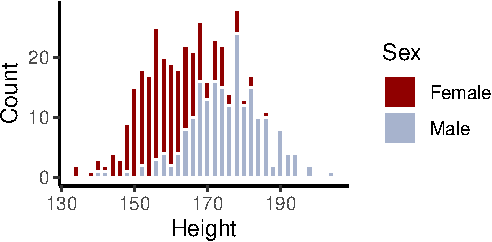
\includegraphics[keepaspectratio]{example_paper_files/figure-pdf/Histogram-1.pdf}}

\vspace{-5pt}
\begin{minipage}{0.9\textwidth}
\scriptsize
\singlespacing
\textbf{Notes:} You can use this text to provide further information about the table. \lipsum[66]
\end{minipage}
\vspace{15pt}

}

\end{figure}%

\lipsum[2-4]

\begin{figure}

\caption{\label{fig-barchart}Number of Federal States by Country}

\centering{

\pandocbounded{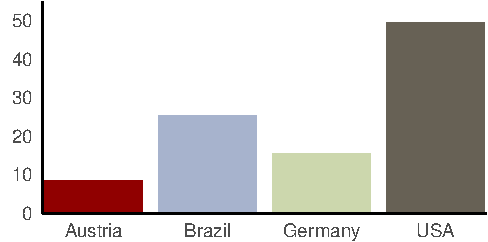
\includegraphics[keepaspectratio]{example_paper_files/figure-pdf/Barchart-1.pdf}}

\vspace{-5pt}
\begin{minipage}{0.9\textwidth}
\scriptsize
\singlespacing
\textbf{Notes:} You can use this text to provide further information about the table. \lipsum[66]
\end{minipage}
\vspace{15pt}

}

\end{figure}%

\lipsum[1-2]

\begin{figure}

\caption{\label{fig-ts1}Displaying how things evolve over time}

\centering{

\pandocbounded{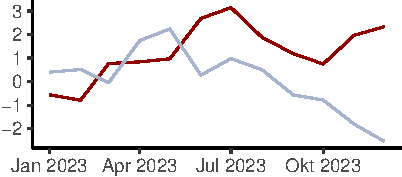
\includegraphics[keepaspectratio]{example_paper_files/figure-pdf/tsplot1-1.pdf}}

\vspace{-5pt}
\begin{minipage}{0.9\textwidth}
\scriptsize
\singlespacing
\textbf{Notes:} You can use this text to provide further information about the table. \lipsum[66]
\end{minipage}
\vspace{15pt}

}

\end{figure}%

\lipsum[1-2]

\begin{figure}

\caption{\label{fig-scatterplot}Two groups have very different values}

\centering{

\pandocbounded{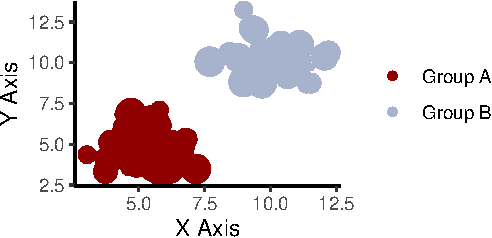
\includegraphics[keepaspectratio]{example_paper_files/figure-pdf/scatterplot-1.pdf}}

\vspace{-5pt}
\begin{minipage}{0.9\textwidth}
\scriptsize
\singlespacing
\textbf{Notes:} You can use this text to provide further information about the table. \lipsum[66]
\end{minipage}
\vspace{15pt}

}

\end{figure}%

\lipsum[1]

\begin{figure}

\caption{\label{fig-dotplot}Visualizing distributions with few
observations}

\centering{

\pandocbounded{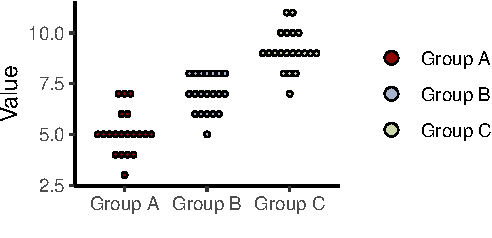
\includegraphics[keepaspectratio]{example_paper_files/figure-pdf/dotplot-1.pdf}}

\vspace{-10pt}
\begin{minipage}{0.9\textwidth}
\scriptsize
\singlespacing
\textbf{Notes:} You can use this text to provide further information about the plot. \lipsum[66]
\end{minipage}
\vspace{15pt}

}

\end{figure}%

\lipsum[1-2]

\begin{figure}

\caption{\label{fig-eventstudy}Coefficients relative to treatment time}

\centering{

\pandocbounded{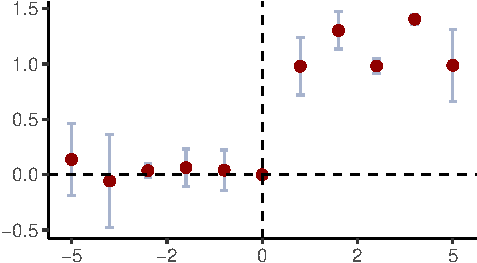
\includegraphics[keepaspectratio]{example_paper_files/figure-pdf/eventstudy-1.pdf}}

\vspace{-7pt}\begin{minipage}{0.9\textwidth}\scriptsize\singlespacing\textbf{Notes:} You can use this text to provide further information about the plot. \lipsum[66]\end{minipage}\vspace{15pt}

}

\end{figure}%

\begin{figure}

\caption{\label{fig-choro}This is a choropleth map}

\centering{

\pandocbounded{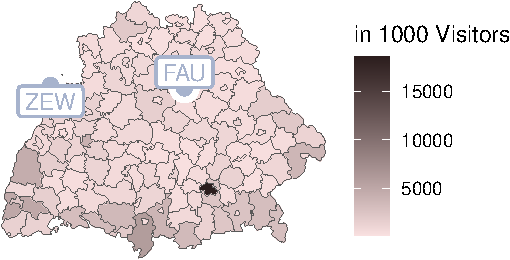
\includegraphics[keepaspectratio]{example_paper_files/figure-pdf/choro-1.pdf}}

\vspace{-10pt}
\begin{minipage}{0.9\textwidth}
\scriptsize
\singlespacing
\textbf{Notes:} You can use this text to provide further information about the table. \lipsum[66]
\end{minipage}
\vspace{15pt}

}

\end{figure}%

\begin{figure}

\caption{\label{fig-indic}This is an indicator map}

\centering{

\pandocbounded{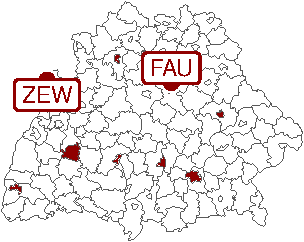
\includegraphics[keepaspectratio]{example_paper_files/figure-pdf/indic-1.pdf}}

\vspace{-10pt}
\begin{minipage}{0.9\textwidth}
\scriptsize
\singlespacing
\textbf{Notes:} You can use this text to provide further information about the table. \lipsum[66]
\end{minipage}
\vspace{15pt}

}

\end{figure}%

\section{Tables}\label{tables}

\lipsum[1-2]
\clearpage

\begin{table}

\caption{\label{tbl-descriptives}Descriptive statistics by group}

\centering{

\fontsize{12.0pt}{14.4pt}\selectfont
\begin{tabular*}{\linewidth}{@{\extracolsep{\fill}}lcc}
\toprule
\textbf{Characteristic} & \textbf{0}, N = 265 & \textbf{1}, N = 235 \\ 
\midrule\addlinespace[2.5pt]
Survival & 0.16 (0.37) & 0.47 (0.50) \\ 
Age in years & 49.86 (16.75) & 50.50 (17.93) \\ 
Female & 0.51 (0.50) & 0.52 (0.50) \\ 
Severity Score & 0.39 (0.49) & 0.36 (0.48) \\ 
\bottomrule
\end{tabular*}
\begin{minipage}{\linewidth}
­\\
\textbf{Notes:} Here is additional information
on the table, which can be lengthy. It does
not have to be but in order to check for line
breaks, it makes sense to have it this way.
It does not have to be but in order to check
for line breaks, it makes sense to have it
this way.\\
\end{minipage}

}

\end{table}%

\lipsum[1-2]
\clearpage

\begin{table}

\caption{\label{tbl-regression}Linear Regression Models}

\centering{

\fontsize{12.0pt}{14.4pt}\selectfont
\begin{tabular*}{\linewidth}{@{\extracolsep{\fill}}lcccccc}
\toprule
 & \multicolumn{2}{c}{Full Sample} & \multicolumn{2}{c}{Men} & \multicolumn{2}{c}{Women} \\ 
\cmidrule(lr){2-3} \cmidrule(lr){4-5} \cmidrule(lr){6-7}
  & (I) & (II) & (III) & (IV) & (V) & (VI) \\ 
\midrule\addlinespace[2.5pt]
Treatment & 0.310*** & 0.299*** & 0.337*** & 0.326*** & 0.284*** & 0.267*** \\ 
{} & {(0.040)} & {(0.038)} & {(0.057)} & {(0.053)} & {(0.055)} & {(0.054)} \\ 
N & 500 & 500 & 242 & 242 & 258 & 258 \\ 
R² & 0.11 & 0.20 & 0.13 & 0.25 & 0.10 & 0.17 \\ 
\bottomrule
\end{tabular*}
\begin{minipage}{\linewidth}
­\\
\textbf{Notes:} Here is additional information on the table, which can be
lengthy. It does not have to be but in order to check for line breaks,
it makes sense to have it this way. It does not have to be but in order
to check for line breaks, it makes sense to have it this way.\\
\end{minipage}

}

\end{table}%

\lipsum[1-2]

\section*{References}\label{references}
\addcontentsline{toc}{section}{References}

\printbibliography[heading=none]

\clearpage

\newpage{}

\section*{Appendix}\label{appendix}
\addcontentsline{toc}{section}{Appendix}

% Always keep this code if you want to use an appendix

\renewcommand{\thetable}{A.\arabic{table}}
\renewcommand{\thefigure}{A.\arabic{figure}}
\setcounter{table}{0}
\setcounter{figure}{0}
\FloatBarrier

\begin{table}

\caption{\label{tbl-regression2}Linear Regression Models for the
Appendix}

\centering{

\fontsize{12.0pt}{14.4pt}\selectfont
\begin{tabular*}{\linewidth}{@{\extracolsep{\fill}}lcccccc}
\toprule
 & \multicolumn{2}{c}{Full Sample} & \multicolumn{2}{c}{Men} & \multicolumn{2}{c}{Women} \\ 
\cmidrule(lr){2-3} \cmidrule(lr){4-5} \cmidrule(lr){6-7}
  & (I) & (II) & (III) & (IV) & (V) & (VI) \\ 
\midrule\addlinespace[2.5pt]
Treatment & 0.310*** & 0.299*** & 0.337*** & 0.326*** & 0.284*** & 0.267*** \\ 
{} & {(0.040)} & {(0.038)} & {(0.057)} & {(0.053)} & {(0.055)} & {(0.054)} \\ 
N & 500 & 500 & 242 & 242 & 258 & 258 \\ 
R² & 0.11 & 0.20 & 0.13 & 0.25 & 0.10 & 0.17 \\ 
\bottomrule
\end{tabular*}
\begin{minipage}{\linewidth}
­\\
\textbf{Notes:} Here is additional information on the table, which can be
lengthy. It does not have to be but in order to check for line breaks,
it makes sense to have it this way. It does not have to be but in order
to check for line breaks, it makes sense to have it this way.\\
\end{minipage}

}

\end{table}%

\begin{figure}

\caption{\label{fig-two}Complex figure with two parts}

\centering{

\begin{figure}[H]

\begin{minipage}{0.50\linewidth}
\subcaption{\label{}Time Series}

\pandocbounded{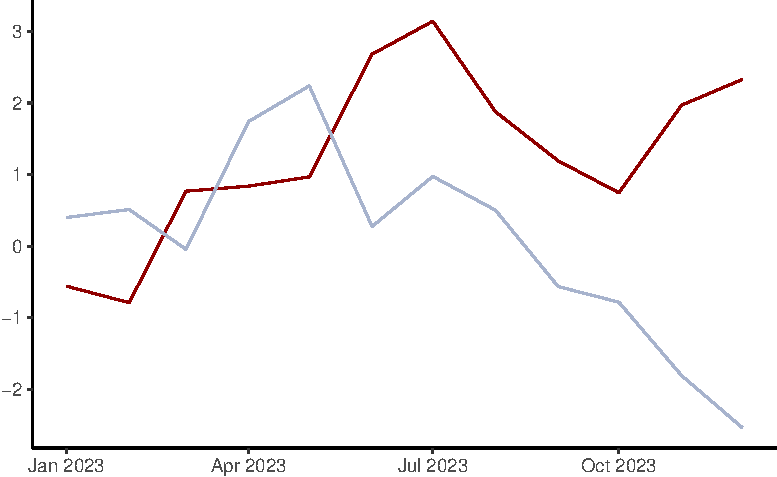
\includegraphics[keepaspectratio]{example_paper_files/figure-pdf/jointplot-1.pdf}}

\end{minipage}%
%
\begin{minipage}{0.50\linewidth}
\subcaption{\label{}Scatterplot}

\pandocbounded{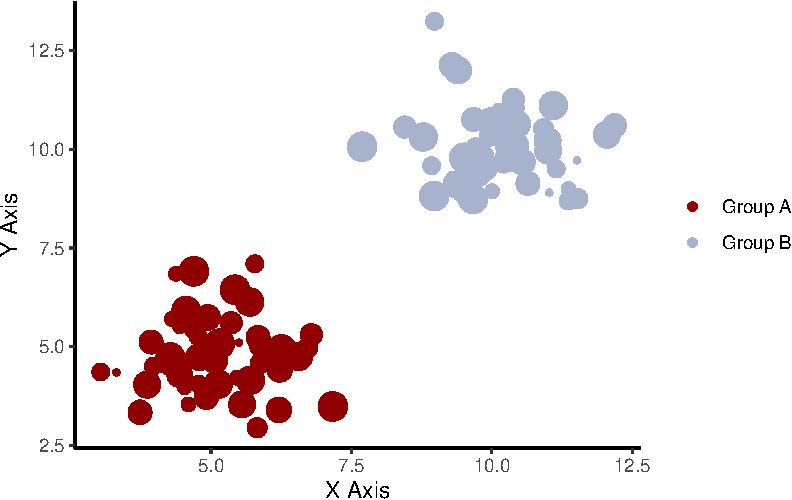
\includegraphics[keepaspectratio]{example_paper_files/figure-pdf/jointplot-2.pdf}}

\end{minipage}%

\end{figure}%

\vspace{-5pt}
\begin{minipage}{0.9\textwidth}
\scriptsize
\singlespacing
\textbf{Notes:} You can use this text to provide further information about the table. \lipsum[66]
\end{minipage}
\vspace{15pt}

}

\end{figure}%

\begin{figure}

\caption{\label{fig-complex}Complex figure with three parts}

\centering{

\begin{figure}[H]

\begin{minipage}{0.45\linewidth}
\subcaption{\label{}Time Series}

\pandocbounded{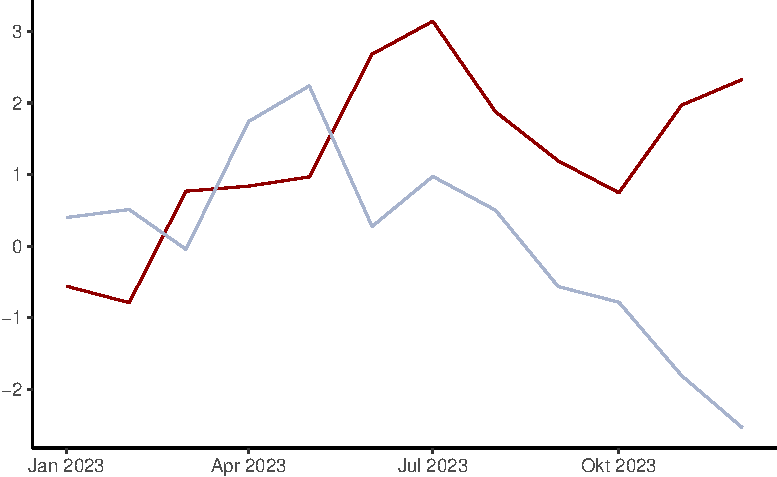
\includegraphics[keepaspectratio]{example_paper_files/figure-pdf/complexplot-1.pdf}}

\end{minipage}%
%
\begin{minipage}{0.10\linewidth}
~\end{minipage}%
%
\begin{minipage}{0.45\linewidth}
\subcaption{\label{}Scatterplot}

\pandocbounded{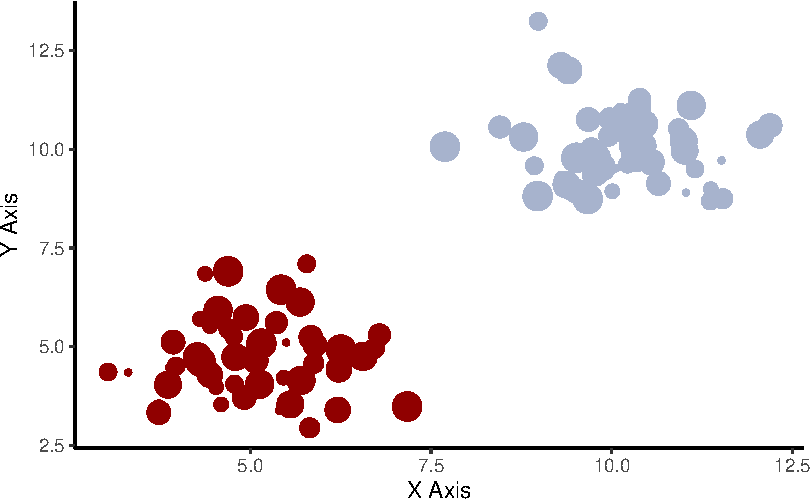
\includegraphics[keepaspectratio]{example_paper_files/figure-pdf/complexplot-2.pdf}}

\end{minipage}%
\newline
\begin{minipage}{\linewidth}
\subcaption{\label{}Histogram}

\pandocbounded{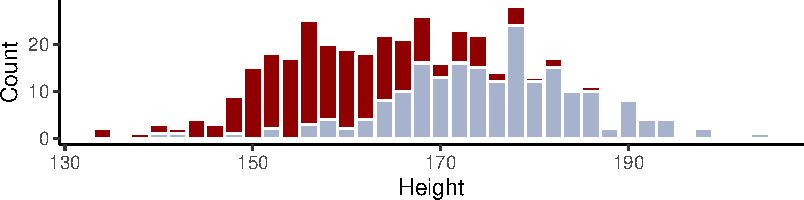
\includegraphics[keepaspectratio]{example_paper_files/figure-pdf/complexplot-3.pdf}}

\end{minipage}%
\newline
\begin{minipage}{0.35\linewidth}
~\end{minipage}%
%
\begin{minipage}{0.30\linewidth}
\pandocbounded{
\includegraphics[keepaspectratio]{example_paper_files/figure-pdf/complexplot-4.pdf}}\end{minipage}%
%
\begin{minipage}{0.35\linewidth}
~\end{minipage}%

\end{figure}%

\vspace{-5pt}
\begin{minipage}{0.9\textwidth}
\scriptsize
\singlespacing
\textbf{Notes:} You can use this text to provide further information about the table. \lipsum[66]
\end{minipage}
\vspace{15pt}

}

\end{figure}%
\end{document}
